\documentclass{simple}

\usepackage{subcaption}

\title[Notele contează]{Notele contează}
\institute{Code Sinaia 2020 (online)}
\author[Răzvan Deaconescu]{Răzvan Deaconescu \\
razvan.deaconescu@cs.pub.ro}
\date{5 august 2020}

\begin{document}

\frame{\titlepage}

\begin{frame}{Note, părinți, profesori}
  \begin{figure}[!htbp]
    \centering
    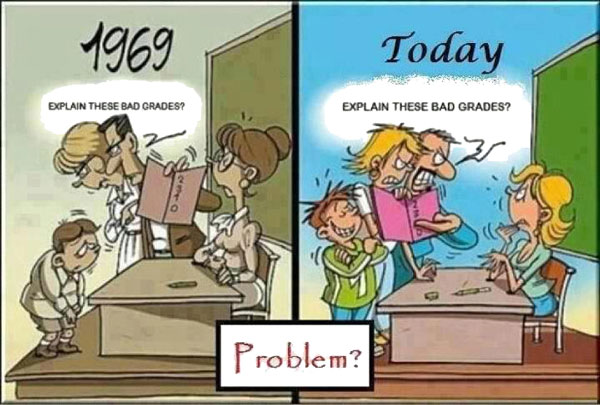
\includegraphics[width=0.8\textwidth]{img/bad-grades.jpg} \\
    \tiny{\url{http://navarre.church/blog-home/2017/1/17/explain-these-bad-grades}}
  \end{figure}
\end{frame}

\begin{frame}{A vs B}
  \centering
  \pause
  \Large
  \textbf{9.50} vs \textbf{8.50} \\
  \pause
  \vspace{3mm}
  \textbf{9.50} vs \textbf{6.50}
\end{frame}

\begin{frame}{Medii mici, dar \ldots}
  \centering
  \pause
  \Large
  Răzvan Nițu \\
  \pause
  \vspace{3mm}
  Cosmin Rațiu
\end{frame}

\begin{frame}{Medii mici, dar \ldots{} (2)}
  \centering
  \pause
  \Large
  Mihai Eminescu \\
  \pause
  \vspace{3mm}
  Albert Einstein
\end{frame}

\begin{frame}{}
  \centering
  \Large
  Excepțiile nu fac regula.
\end{frame}

\begin{frame}{}
  \centering
  \Large
  Contează notele?
\end{frame}

\begin{frame}{}
  \centering
  \Large
  Când \textbf{nu} contează notele?
\end{frame}

\begin{frame}{}
  \centering
  \Large
  Când contează notele?
\end{frame}

\begin{frame}{}
  \pause
  \centering
  \Large
  good nerd vs bad nerd \\
  \pause
  \vspace{3mm}
  tocilar bun vs tocilar rău
\end{frame}

\begin{frame}{Notele ca metrică}
  \textit{Nu poți avea performanță fără evaluare}. \\
  \vspace{3mm}
  \hfill \textit{Valentin Cristea}
\end{frame}

\begin{frame}{Notele ca metrică (2)}
  \textit{Winners forget they're in a race, they just love to run.} \\
  \vspace{3mm}
  \hfill \textit{Simon Wilder (With Honors, 1994)}
\end{frame}

\begin{frame}{Ca un fel de concluzie}
  \centering
  \pause
  Nu gândiți binar, gândiți nuanțat. \\
  \vspace{3mm}
  \pause
  Notele sunt o metrică, nu un obiectiv. \\
  \vspace{3mm}
  \pause
  It's more about the journey than the destination. \\
  \vspace{3mm}
  \pause
  \textbf{Notele contează, dar nu în absolut.}
\end{frame}

\begin{frame}{Decizii grele și decizii ușoare}
  \scriptsize
  \url{https://seths.blog/2020/08/two-kinds-of-decisions-worth-focusing-on/}
\end{frame}

\begin{frame}{Resurse}
  \begin{itemize}
    \item slide-urile prezentării: \url{https://www.slideshare.net/razvandeaconescu/}
    \item Doru Căstăian (doru.castaian) (Facebook)
    \item Richard Feynman (@ProfFeynman) (Twitter)
    \item James Clear (@JamesClear) (Twitter)
    \item Seth Godin (@ThisIsSethsBlog) (Twitter)
    \item \url{https://seths.blog/}
  \end{itemize}
\end{frame}

\end{document}
